\documentclass[11pt]{article}
\usepackage[a4paper,landscape,margin=0.72in]{geometry}
\usepackage[T1]{fontenc}
\usepackage{lmodern,amsmath,amssymb,graphicx,hyperref}
\title{Rational nonbranch point: principal ideal and actual DVR}
\author{Formal proof packet}
\date{28 October 2026}
\begin{document}
\maketitle
\noindent This packet records a checked local geometry theorem. It contains no experiment, target result, or cost ratio. The Lean source, compiler log, editable SVG, and CSV gate table accompany this PDF.

\section*{Checked boundary}
Let $K$ be any field, $f(X)=X^5+a_3X^3+a_2X^2+a_1X+a_0$, and $(a,y)\in K^2$ satisfy $y^2=f(a)$. Assume $f$ is separable and $2y\ne0$. The point evaluation ideal in $K[X,Y]/(Y^2-f(X))$ is $(X-a,Y-y)$. In the localization at this ideal, $Y+y$ is a unit because its residue is $2y$. The curve relation gives
\[
  (Y-y)(Y+y)=(X-a)q_a(X).
\]
Thus the local maximal ideal is generated by $X-a$. This generator is nonzero, and the separability bridge already proves that the affine coordinate ring and localization are domains. The checked DVR criterion gives a discrete valuation ring. The checked ring equivalence transports this structure to the \emph{actual weighted-$\operatorname{Proj}$ point stalk}.

\section*{Scope and verification}
The condition $2y\ne0$ is essential for this proof and cannot be replaced by $y\ne0$ in characteristic two. Over $\mathbf F_2$, $f=X^5+X^3+1$ is separable, yet $(0,1)$ is on the curve and both partial derivatives vanish there. The alternate pointwise case $f'(a)\ne0$ is not formalized here.

The direct pinned Lean 4.34.1 compile exited zero against Mathlib revision
\par\noindent\texttt{d13f23b723b8a846827a245b89c10fc7d3f11612}.
Ten printed axiom audits list only \texttt{propext}, \texttt{Classical.choice}, and \texttt{Quot.sound}; no \texttt{sorryAx}. Lean source SHA-256:
\par\noindent{\small\texttt{0eb48894992f0c1e412c20cdec44acc71692ea2b165b2d7afc3d72b6b204ce3f}}.
The compiler log retains nonfatal style-linter suggestions. The local DVR criterion is the pinned Mathlib \texttt{IsDiscreteValuationRing.TFAE}, corresponding to Stacks Project Tag 00PD. Stalk transport uses the prior checked open-immersion equivalence, corresponding to Stacks Tag 01HD.

Formula-specific norm transport into this stalk remains open, as do global principal-divisor/$\mathrm{Pic}^0$ transport and compiled Rust semantics. The CSV gives the exact status of each theorem and gate.

\clearpage
\section*{Proof dependencies and open gates}
\begin{center}
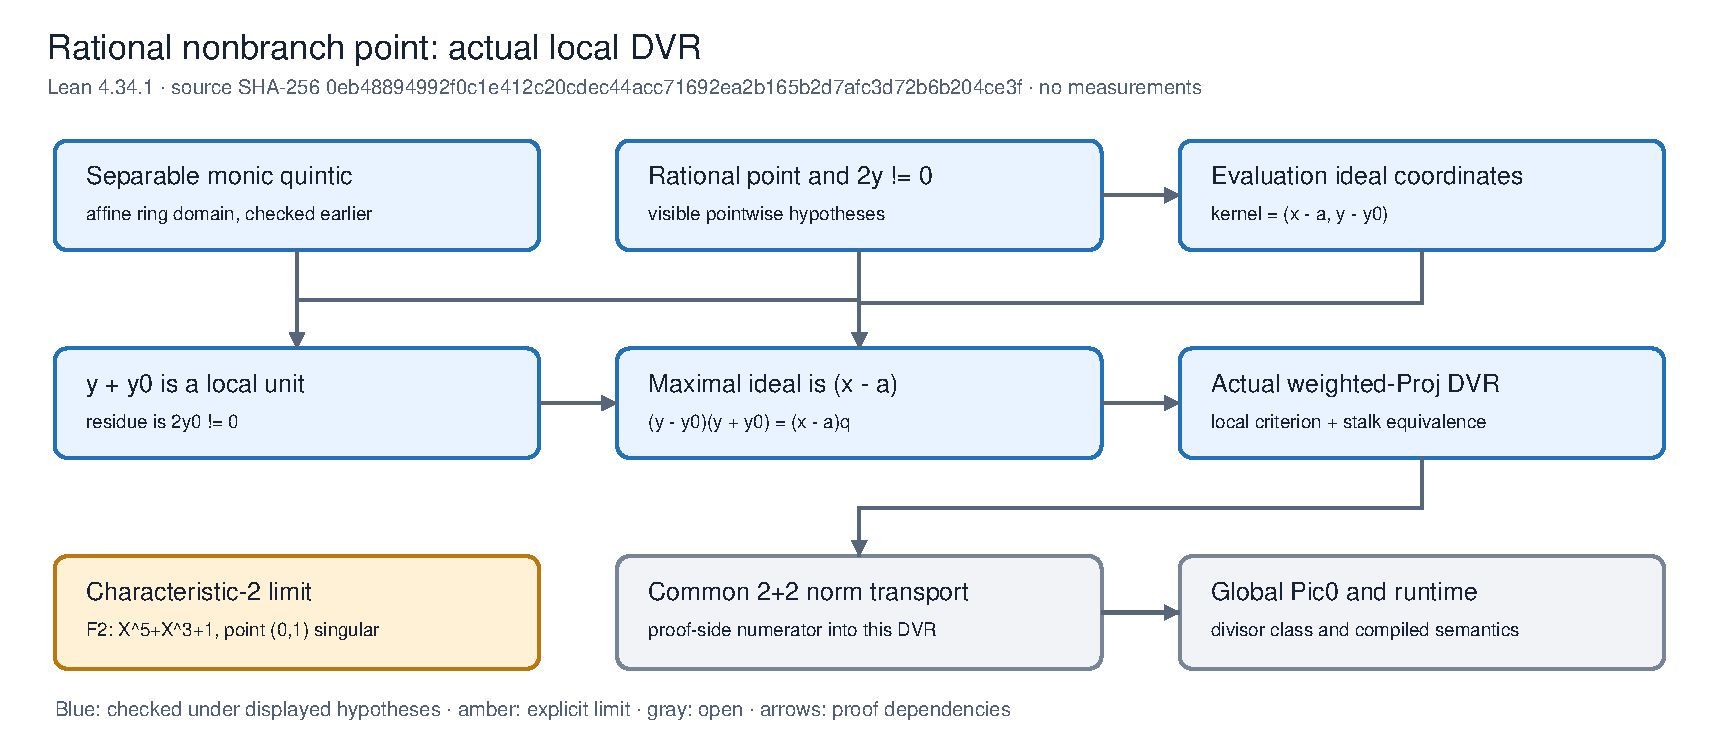
\includegraphics[width=0.96\textwidth,height=0.76\textheight,keepaspectratio]{nonbranch-dvr-figure.pdf}
\end{center}
\noindent Blue nodes are checked under the displayed hypotheses. Amber records the characteristic-two limit; gray nodes are open. Arrows show proof dependencies, not measured performance.
\end{document}
